\begin{answer}
    \begin{figure}[htbp]
        \begin{subfigure}[b]{0.5\linewidth}
            \centering
            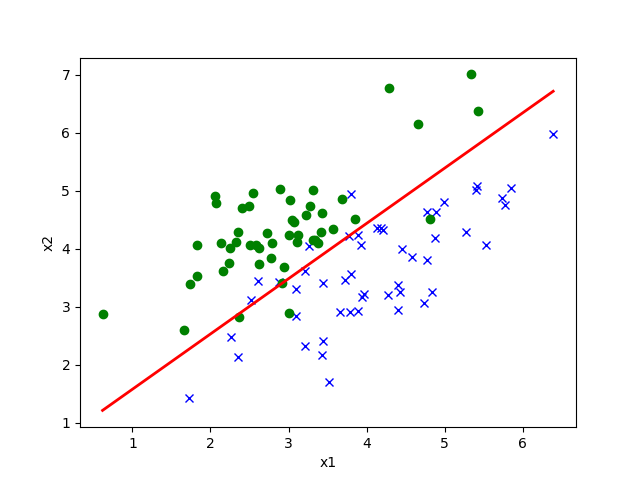
\includegraphics[width=\linewidth]{../src/output/p01b_pred_2.png}
            \subcaption{Logistic Regression on Dataset 2}
        \end{subfigure}
        \begin{subfigure}[b]{0.5\linewidth}
            \centering
            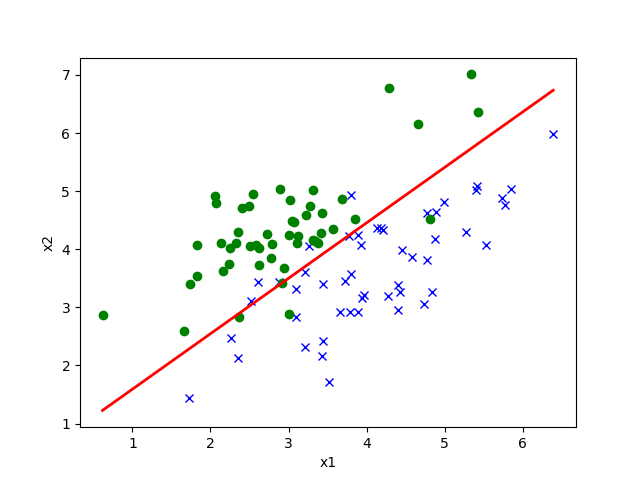
\includegraphics[width=\linewidth]{../src/output/p01e_pred_2.png}
            \subcaption{GDA on Dataset 2}
        \end{subfigure}
    \end{figure}
    \\GDA makes stronger assumptions, including assuming a gaussian distribution.\\
    Therefore we can see the reason it's less effective on Dataset 1
\end{answer}
